%% BioMed_Central_Tex_Template_v1.06
%%                                      %
%  bmc_article.tex            ver: 1.06 %
%                                       %

%%IMPORTANT: do not delete the first line of this template
%%It must be present to enable the BMC Submission system to
%%recognise this template!!

%%%%%%%%%%%%%%%%%%%%%%%%%%%%%%%%%%%%%%%%%
%%                                     %%
%%  LaTeX template for BioMed Central  %%
%%     journal article submissions     %%
%%                                     %%
%%          <8 June 2020>              %%
%%                                     %%
%%                                     %%
%%%%%%%%%%%%%%%%%%%%%%%%%%%%%%%%%%%%%%%%%

%%%%%%%%%%%%%%%%%%%%%%%%%%%%%%%%%%%%%%%%%%%%%%%%%%%%%%%%%%%%%%%%%%%%%
%%                                                                 %%
%% For instructions on how to fill out this Tex template           %%
%% document please refer to Readme.html and the instructions for   %%
%% authors page on the biomed central website                      %%
%% https://www.biomedcentral.com/getpublished                      %%
%%                                                                 %%
%% Please do not use \input{...} to include other tex files.       %%
%% Submit your LaTeX manuscript as one .tex document.              %%
%%                                                                 %%
%% All additional figures and files should be attached             %%
%% separately and not embedded in the \TeX\ document itself.       %%
%%                                                                 %%
%% BioMed Central currently use the MikTex distribution of         %%
%% TeX for Windows) of TeX and LaTeX.  This is available from      %%
%% https://miktex.org/                                             %%
%%                                                                 %%
%%%%%%%%%%%%%%%%%%%%%%%%%%%%%%%%%%%%%%%%%%%%%%%%%%%%%%%%%%%%%%%%%%%%%

%%% additional documentclass options:
%  [doublespacing]
%  [linenumbers]   - put the line numbers on margins

%%% loading packages, author definitions

%\documentclass[twocolumn]{bmcart}% uncomment this for twocolumn layout and comment line below
\documentclass{bmcart}
\usepackage{hyperref}

%%% Load packages
\usepackage{tabularx}
\usepackage{multirow}
\usepackage{lscape}
\usepackage{rotating}
\usepackage{amsthm,amsmath}
%\RequirePackage[authoryear]{natbib}% uncomment this for author-year bibliography
%\RequirePackage{hyperref}
\usepackage{graphicx}
\usepackage[utf8]{inputenc} %unicode support
%\usepackage[applemac]{inputenc} %applemac support if unicode package fails
%\usepackage[latin1]{inputenc} %UNIX support if unicode package fails

%%%%%%%%%%%%%%%%%%%%%%%%%%%%%%%%%%%%%%%%%%%%%%%%%
%%                                             %%
%%  If you wish to display your graphics for   %%
%%  your own use using includegraphic or       %%
%%  includegraphics, then comment out the      %%
%%  following two lines of code.               %%
%%  NB: These line *must* be included when     %%
%%  submitting to BMC.                         %%
%%  All figure files must be submitted as      %%
%%  separate graphics through the BMC          %%
%%  submission process, not included in the    %%
%%  submitted article.                         %%
%%                                             %%
%%%%%%%%%%%%%%%%%%%%%%%%%%%%%%%%%%%%%%%%%%%%%%%%%

%\def\includegraphic{}
%\def\includegraphics{}

%%% Put your definitions there:
\startlocaldefs
\endlocaldefs

%%% Begin ...
\begin{document}

%%% Start of article front matter
\begin{frontmatter}

\begin{fmbox}
\dochead{Research}

%%%%%%%%%%%%%%%%%%%%%%%%%%%%%%%%%%%%%%%%%%%%%%
%%                                          %%
%% Enter the title of your article here     %%
%%                                          %%
%%%%%%%%%%%%%%%%%%%%%%%%%%%%%%%%%%%%%%%%%%%%%%

\title{Predicting Comperhensive Drug - Drug Interaction via Similarity Network Fusion and Convolutional Neural Networks}

%%%%%%%%%%%%%%%%%%%%%%%%%%%%%%%%%%%%%%%%%%%%%%
%%                                          %%
%% Enter the authors here                   %%
%%                                          %%
%% Specify information, if available,       %%
%% in the form:                             %%
%%   <key>={<id1>,<id2>}                    %%
%%   <key>=                                 %%
%% Comment or delete the keys which are     %%
%% not used. Repeat \author command as much %%
%% as required.                             %%
%%                                          %%
%%%%%%%%%%%%%%%%%%%%%%%%%%%%%%%%%%%%%%%%%%%%%%
\author[
  addressref={aff1,aff2},
  email={khodamoradi1992@gmail.com}
]{\inits{M.A.K.}\fnm{Mohammad.Amin} \snm{Khodamoradi}}
\author[
  addressref={aff1,aff2},
  email={Bahar.levian@gmail.com}
]{\inits{B.L.}\fnm{Bahareh} \snm{Levian}}
\author[
  addressref={aff1,aff2},                   % id's of addresses, e.g. {aff1,aff2}
  corref={aff1},                       % id of corresponding address, if any
% noteref={n1},                        % id's of article notes, if any
  email={eslahchi.ch@gmail.com}   % email address
]{\inits{C.E.}\fnm{Changiz} \snm{Eslahchi}}


%%%%%%%%%%%%%%%%%%%%%%%%%%%%%%%%%%%%%%%%%%%%%%
%%                                          %%
%% Enter the authors' addresses here        %%
%%                                          %%
%% Repeat \address commands as much as      %%
%% required.                                %%
%%                                          %%
%%%%%%%%%%%%%%%%%%%%%%%%%%%%%%%%%%%%%%%%%%%%%%

\address[id=aff1]{%                           % unique id
  \orgdiv{Department of Computer Science},             % department, if any
  \orgdiv{Faculty of Mathematical Science},
  \orgname{Shahid Beheshti University},          % university, etc
  \city{Tehran},                              % city
  \cny{Iran}                                    % country
}
\address[id=aff2]{%
  \orgdiv{School of Bioinformatics},
  \orgname{IPM - Institute for Research in Fundamental Sciences},
  %\street{},
  %\postcode{}
  \city{Tehran},                              % city
  \cny{Iran}
}

%%%%%%%%%%%%%%%%%%%%%%%%%%%%%%%%%%%%%%%%%%%%%%
%%                                          %%
%% Enter short notes here                   %%
%%                                          %%
%% Short notes will be after addresses      %%
%% on first page.                           %%
%%                                          %%
%%%%%%%%%%%%%%%%%%%%%%%%%%%%%%%%%%%%%%%%%%%%%%

%\begin{artnotes}
%%\note{Sample of title note}     % note to the article
%\note[id=n1]{Equal contributor} % note, connected to author
%\end{artnotes}

\end{fmbox}% comment this for two column layout

%%%%%%%%%%%%%%%%%%%%%%%%%%%%%%%%%%%%%%%%%%%%%%%
%%                                           %%
%% The Abstract begins here                  %%
%%                                           %%
%% Please refer to the Instructions for      %%
%% authors on https://www.biomedcentral.com/ %%
%% and include the section headings          %%
%% accordingly for your article type.        %%
%%                                           %%
%%%%%%%%%%%%%%%%%%%%%%%%%%%%%%%%%%%%%%%%%%%%%%%

\begin{abstractbox}

\begin{abstract} % abstract
\parttitle{Background} %if any
Drug-drug interactions (DDIs) always cause unexpected and even adverse drug reactions. It is important to identify DDIs before drugs are used in the market.However, preclinical identification of DDIs requires much money and time. Computational approaches have exhibited their abilities to predict potential DDIs on a large scale by utilizing premarket drug properties. Nevertheless, most of them only predict whether or not one drug interacts with another, but neglect their enhancive (positive) and depressive (negative) changes of pharmacological effects. Moreover, these comprehensive DDIs do not occur at random, and derived from the structural features of the graph of DDIs. Revealing such a relationship is very important, because it is able to help understand how DDIs occur. Both the prediction of comprehensive DDIs and the discovery of structural relationship among them play an important guidance when making a co-prescription.

\parttitle{Results} %if any
In this work, treating a set of comprehensive DDIs as a signed network, we design a novel model (SNF-CNN) for the prediction of enhancive and degressive DDIs based on similarity network fusion and convolutional neural networks. SNF-CNN achieves the depressive DDI prediction ($AUC=0/9747 \pm 0/0033 $ and $AUPR=0/9666 \pm 0/0045 $), enhancive DDI prediction ($AUC=0/9686 \pm 0/0028$ and $AUPR=0/8221 \pm 0/0184$) and the Unknown DDI prediction ($AUC=0/9714 \pm 0/0040$ and $AUPR=0/9480 \pm 0/0083$). Compared with three state-of-the-art approaches, SNF-CNN shows it superiority.

\parttitle{Conclusions} %if any
This new approach is not only able to predict comprehensive DDI, but also predicts non-DDI.
\end{abstract}

%%%%%%%%%%%%%%%%%%%%%%%%%%%%%%%%%%%%%%%%%%%%%%
%%                                          %%
%% The keywords begin here                  %%
%%                                          %%
%% Put each keyword in separate \kwd{}.     %%
%%                                          %%
%%%%%%%%%%%%%%%%%%%%%%%%%%%%%%%%%%%%%%%%%%%%%%

\begin{keyword} 
\kwd{Drug-Drug Interaction}
\kwd{Drug Similarity}
\kwd{Drug Similarity Integration}
\kwd{Feature Selection}
\kwd{Recommender System}
\end{keyword}

% MSC classifications codes, if any
%\begin{keyword}[class=AMS]
%\kwd[Primary ]{}
%\kwd{}
%\kwd[; secondary ]{}
%\end{keyword}

\end{abstractbox}
%
%\end{fmbox}% uncomment this for two column layout

\end{frontmatter}

%%%%%%%%%%%%%%%%%%%%%%%%%%%%%%%%%%%%%%%%%%%%%%%%
%%                                            %%
%% The Main Body begins here                  %%
%%                                            %%
%% Please refer to the instructions for       %%
%% authors on:                                %%
%% https://www.biomedcentral.com/getpublished %%
%% and include the section headings           %%
%% accordingly for your article type.         %%
%%                                            %%
%% See the Results and Discussion section     %%
%% for details on how to create sub-sections  %%
%%                                            %%
%% use \cite{...} to cite references          %%
%%  \cite{koon} and                           %%
%%  \cite{oreg,khar,zvai,xjon,schn,pond}      %%
%%                                            %%
%%%%%%%%%%%%%%%%%%%%%%%%%%%%%%%%%%%%%%%%%%%%%%%%

%%%%%%%%%%%%%%%%%%%%%%%%% start of article main body
% <put your article body there>

%%%%%%%%%%%%%%%%
%% Background %%
%%
\section*{Introduction}
When two or more drugs are taken together, drugs' effects or behaviors are unexpectedly influenced by each other
\cite{wienkers2005predicting}. 
This kind of influence is termed as Drug-Drug interaction (DDI), which would reduce drug efficacy, increase unexpected toxicity, or induce other adverse drug reactions between the co-prescribed drugs. As the number of approved drugs increases, the number of drug-unidentified DDIs is rapidly increasing, such that among approved small molecular drugs in Drug Bank, on average, 15 out of every 100  drug pairs have DDIs
\cite{law2014drugbank}. 
The DDIs would put patients who are treated with multiple drugs in an unsafe situation
\cite{leape1995systems, businaro2013we, karbownik2017pharmacokinetic, mulroy2017giant}.
Understanding DDI is the first step in drug combinations, which becomes one of the most promising solutions for the treatment of multifactorial complex diseases
\cite{zhao2011prediction}.
Therefore, there is an urgent need for screening and analysis of DDIs before clinical co-medications are administered. However, traditional DDI identification approaches (e.g., testing Cytochrome P450
\cite{veith2009comprehensive}
 or transporter-associated interactions
\cite{huang2007drug})
face challenges, such as high costs, long duration, animal welfare considerations
\cite {zhang2015label},
the very limited number of participants in the trial, and the great number of drug combinations under screening in clinical trials. As a result, only a few DDIs have been identified during drug development production (usually in the clinical trial phase). Some of them have been reported after drugs approved, and many have been found in post-marketing surveillance.

Computational approaches are a promising alternative to discovering potential DDIs on a large scale, and they have gained attention from academy and industry recently
\cite{wisniowska2016role, zhou2016simulation}.
Data mining-based computational approaches have been developed to detect DDIs from various sources
\cite{zhang2015label}
, such as scientific literature
\cite{bui2014novel, zhang2016leveraging}
, electronic medical records
\cite{yamanishi2008prediction}
, and the Adverse Event Reporting System of FDA (http://www.fda.gov). These approaches rely on post-market clinical evidence. So, they cannot provide alerts of potential DDIs before clinical medications are administered. In contrast, machine learning-based computational approaches (e.g. Naïve Similarity-Based Approach
\cite{vilar2014similarity}
, Network Recommendation-Based
\cite{zhang2015label}
, Classification-Based
\cite{cheng2014machine}
) can provide such alerts by utilizing pre-marketed or post-marketed drug attributes, such as drug features or similarities
\cite{pahikkala2015toward}.
These methods use different drug features to predict DDIs, such as chemical structures
\cite{vilar2014similarity}
, targets
\cite{luo2014ddi}
, hierarchical classification codes
\cite{cheng2014machine}
, side effects, and off-label side effects
\cite{zhang2015label, shi2017predicting}.

Most of these existing machine learning approaches are designed to predict the typical two-class problem, which only indicates how likely a pair of drugs is a DDI. However, two interacting drugs may change their own pharmacological behaviors or effects (e.g., increasing or decreasing serum concentration) in vivo. For example, the serum concentration of Flunisolide (DrugBank Id: DB00180) decreases when it is taken with Mitotane (DrugBank Id: DB00648), whereas its serum concentration increases when taken with Roxithromycin (DrugBank Id: DB00778). For short, the first case is degressive DDI, and the second case is enhancive DDI, which contains drug changes in terms of pharmacological effects. It is more important to know exactly whether the interaction increases or decreases the drug's pharmaceutical behaviors, especially when making optimal patient care, establishing drug dosage, designing prophylactic drug therapy, or finding the resistance to therapy with a drug
\cite{koch1981serum}.

On the other hand, the occurrence of both enhancive and degressive DDIs is not random, but most current approaches have not yet exploited this structural property and have been developed only for conventional two-classes DDIs. Furthermore, revealing such a structural relationship is very important because it can help us understand how DDIs occur. It is one of the most important steps for treating complex diseases and guides physicians in preparing safer prescriptions to high-order drug interaction. The proposed algorithms for predicting three-classes DDIs are introduced in the following. And how they work are briefly described. All three introduced algorithms use matrix factorization methods, which is a network recommender-based approach. The matrix factorization approach, with slightly modifying, is a suitable solution for the subject of predicting DDI that has received much attention from researchers.

In this paper, we firstly introduce data and features. Then, a novel algorithm (SNF-CNN) based on the integration of drug similarities and deep learning recommendation systems for predicting DDI is presented in a comprehensive three-class model. This algorithm is called Predicting Comprehensive Drug-Drug Interaction via Similarity Network Fusion and Convolutional Neural Networks.

The paper is organized as follows. In the first section, the data preparation process is explained. The recommendation system is then designed and trained on enhancive and degressive, which detects pairs of non-interacting drugs with high probability. Next, the previous recommender system, based on a convolutional neural network, is trained on incremental and decremental interaction data without interaction (detected in the previous step).In section Results and Discussions, we investigate the results of SNF-CNN in the 10-fold cross-validation process(10-fold CV).

It should be noted that the proposed method of this research is a recommender-based on deep neural networks and has no structural similarities with matrix factorization methods. The only reason for mentioning these methods is the limited number of articles that have used three-class data in their work.

\section*{Methods}
\subsection*{Dataset and features}
In this study, we use the data set presented in paper of \cite{yu2018predicting}. This set contains 568 approved small molecule drugs, each of them has at least one interaction with the other drugs in the set. In total, the interactions between these 568 drugs contain 21,351 DDIs, including 16,757 enhancive DDIs and 4,594 degressive DDIs.In addition, each drug represented as an  881-dimensional feature vector $ F_ {str} $  based on PubChem chemical structure descriptor and also a 9149-dimensional feature vector $ F_ {se} $ according to the off-label side effects provided by OFFSIDES.

\subsection*{Problem formulation}

Without loss of generality, let $D = \{d_i\}$, $i = 1, 2, .., m$ be a set of m approved drugs. Their  interactions can be accordingly represented as an $m \times m$ symmetric interaction matrix $A_{m \times m} = \{a_{ij}\}$. For the conventional DDIs, $a_{ij} = 1$ if $d_i$ interacts with $d_j$, and $a_{ij} = 0$ otherwise. For the comprehensive DDIs, $a_{ij} \in \{-1, 0, +1\}$ . Again, if $d_i$ and $d_j$ do not interact with each other, $a_{ij} = 0$ . When there is an enhancive DDI or a degressive DDI between $d_i$ and $d_j$ , $a_{ij} = +1$ or $a_{ij} = -1$ respectively.

In addition, each drug $d_i$ in the D is represented as a p-dimension feature vector $f_i = \left[  f_1, f_2, .., f_k, .., f_p \right]$, which $f_k = 1$ indicates the K-th specific chemical structure fragment or occurs an off-label side effect, and $f_k = 0$ otherwise. Because each drug has two chemical structure feature vectors and off-label side effects, there are two feature matrices of $F$ with dimensions of $m \times p$ (amount of p depends on kind of feature ). Matrices of $F_{str}$ and $F_{se}$ are, respectively, the feature matrix of the chemical structure and the feature matrix of off-label side effects.

\subsection*{Data preparing}
Since the new drugs are isolated nodes in the interaction network, we cannot infer their possible interaction from topological information alone. Therefore, additional information (such as chemical structure or off-label side effects) is needed, which is called a drug feature in terms of machine learning. First, we prepare the features based on our model, and then we teach a deep learning model of interaction prediction.

\subsubsection*{Similarity matrix calculation}

A common method of calculating similarity called Cosine Similarity is used in machine learning articles such as Articles \cite{zhang2016drug, zhang2018manifold}. If we name feature vectors of the drug of $d_i$ and $d_j$
as $x_i$ and $x_j$,Cosine Similarity between $x_i$ and $x_j$ is defined as follows:
\begin{equation}
	\begin{aligned}
		S_{Cos}(x_i,x_j) =\dfrac{x_i . x_j}{||x_i||_2 ||x_j||_2}
	\end{aligned}
\end{equation}
Where $||.||_2$ is the Euclidean Norm and ${x_i . x_j}$ is inner product of two vectors.

It was observed that the values of the feature matrices are discrete, and also the dimensions of the matrices are large. The chemical structure and the off-label side effect have 881 and 9149 dimensions, respectively. On the other hand, machine learning algorithms do not work properly with high-dimensional data and discrete data. As a result, they do not get good results on these kinds of data. Therefore, by exploiting the cosine similarity, that was described above, drug similarity matrices based on chemical structure and off-label side effects are calculated. These matrices are $S_{str}$ and $S_{se}$, respectively. The dimensions of these two matrices are $m \times m$, where $s_{i,j}$ is an element of similarity matrices that shows similarity value between drugs of $di$ and $d_j$. Each element of $S$ has a continuous value between zero and one.

\subsubsection*{Integration drug similarity matrices}
Similarity Network Fusion (SNF)\cite{wang2014similarity} is a new computational method for data integration.  Briefly, SNF combines many different types of features (such as chemical structure and off-label side effect, and more - clinical data, questionnaires, image data, etc.) for a given set of samples (e.g., drugs). SNF first constructs a sample similarity network for each of the data types and then iteratively integrates these networks using a novel network fusion method. Working in the sample network space allows SNF to avoid dealing with different scales, collection bias, and noise in different data types. Integrating data in a non-linear fashion allows SNF to take advantage of the common and complementary information in different data types. Figure \ref{fs8} is a good visualization of SNF processes  that has been used in our method structure.

\begin{figure}[!h]
	%\centering
	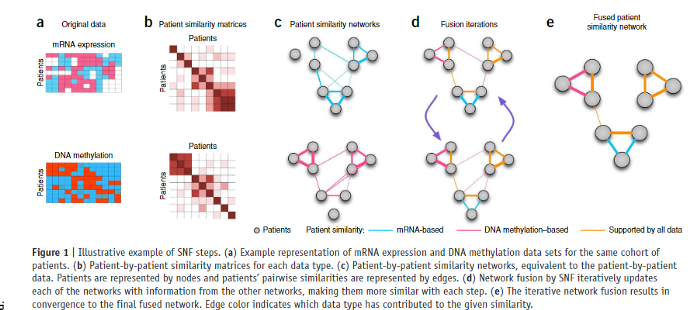
\includegraphics[scale=.53]{SNF.png}
	\caption{SNF processes \cite{wang2014similarity}:
	A detailed example of SNF steps. (a) An example representation of chemical structure feature and off-label side effect feature for the same set of drugs. (b) Drug-drug similarity matrices for each feature type. (c) Drug-drug similarity networks, equivalent to the drug-drug data. Nodes represent drugs, and edges represent drug pairwise similarities. (d) Network fusion by SNF iteratively updates each of the networks with information from the other networks, making them more similar with each step. (e) The iterative network fusion results in convergence to the final fused network. Edge color indicates which data type has contributed to the given similarity. }
	\label{fs8}
\end{figure}

In this section, using the similarity network fusion method that has described above, similarity matrices of the chemical structure and the off-label side effect of drugs were integrated. The output of this integration is a new similarity matrix of $S_{snf}$ with dimensions of $568 \times 568$, and elements of $S_{snf}$ have a value between zero and one.To integrate the network similarity, the package of SNFPy is used, which is implemented in Python and is available at \cite{SNFPy2020}.

\subsubsection*{Input matrix format}

At this stage, a matrix forms with 1139 columns and 322056 rows, which consists of the following columns:

1) Drug pairs: Name of the drug i-th and the name of the drug j-th.

2) Type of interaction: degressive (-1), enhancive (+1), and unknown (0).

3) The similarity vector of i-th drug from the $S_{snf}$ matrix with 568 elements.

4) The similarity vector of j-th drug from the $S_{snf}$ matrix with 568 elements.

Figure of \ref{BMatHeader} shows the header of matrix.

\begin{figure}[!h]
	\centering
	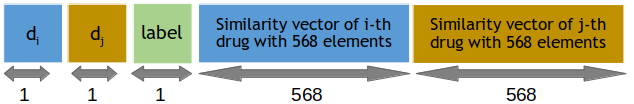
\includegraphics[scale=.53]{MatrixheaderB.png}
	\caption{Matrix header of B}
	\label{BMatHeader}
\end{figure}

We have 568 drugs, and the interaction of each drug with itself is meaningless. On the other hand, the drug pairs of $(d_i, d_j)$ and $(d_j, d_i)$ have the same label, while the corresponding similarity vectors of drugs in the drug pairs have been displaced. So, these drug pairs are dual. Both of them in the data augment the training data, which increases the model's ability to have a better prediction. As a result, the resulting matrix has 322056 data samples or rows ($(568 \times 568) - 568 = 322056$). According to the explanations provided, a matrix with dimensions of $322056 \times 1139$ is formed to input into our model, which is called $B$.

\subsection*{Devising Recommender System}
In the previous steps, data was prepared to input any learning machine models, including deep learning models. Before presenting the model and inputting the data into the machine, one important point must be considered. As discussed, the enhancive and degressive drug pairs have clear and significant labels, while a zero label drug pair does not mean that there is no interaction between them. It indicates, still, no interaction has been found for this pair of drugs. In the following, we present a method for detecting non-interaction drug pairs. Then we use these pairs of drugs as zero-labeled data to train a model in the next phase.

\subsection*{Selecting and training model with known interactions}
To solve this problem, it is necessary to provide a model that detects non-interaction with high accuracy and confidence. Therefore, we design a model based on deep learning that predicts the possible non-interaction drug pairs and then uses them to train a three-class model. Obviously, the higher accuracy in detecting zeros, the more accurate and confident the three-class model will be designed and trained.

\subsubsection*{Cross-validation process for model selection}
We separate rows of matrix B that contain positive or negative interactions. The new matrix contains 42,702 drug pairs with degressive and enhancive interactions. This data was exploited to design more accurate and more efficient network architecture. The obtained data contains 42702 drug pairs, and each pair of drugs has a feature vector with 1136 dimensions. At first, the drug pairs are divided into 10 almost equal parts randomly. Then in 10 iterations (K = 10), in each iteration, one part of data is considered as a test dataset and the other nine parts as a train dataset. The drug pairs of $(d_i, d_j)$ and $(d_j, d_i)$ are not biologically different, so a drug pair and its dual must be in the same part When the data is separated into ten parts. This prevents fraud and improves model training by augmenting the train data.

We tried different models, then trained and evaluated them in the 10-Fold cross-validation procedure. The final model is a deep neural network that is a stack of convolutional and fully connected layers.

\subsubsection*{Presenting the selected model}
\begin{figure}[!h]
	\centering
	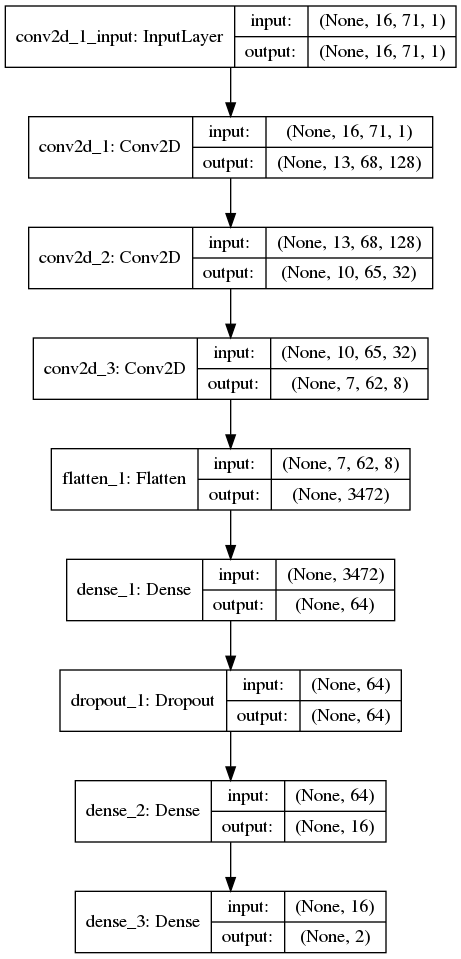
\includegraphics[scale=0.43]{ModelSelection/model(-1,1).png}
		\caption{Layers of CNN model which trains on degressive and enhancive pairs only}
	\label{CNNModel}
\end{figure}
After trying different structures, we have the final deep neural network as shown in Figure
\ref{CNNModel}. This network has three two-dimensional convolution layers. Following them, there are three fully connected convolution layers. The last layer has two outputs for predicting degressive or enhancive interaction. Convolution layers have square filters with a size of $4 \times 4$ and stride of 1. Each convolution layer also has a Relu activation function. The number of convolution filters is 128, 32, and 8, respectively. All connected layers have 64, 16, and 2 nodes, respectively, the first two layers have Relu activation function and the last layer with 2 nodes has a Sigmoid activation function. Convolution layers using a Flatten layer Connects to fully connected layers. The function of this layer is to transform a two-dimensional matrix into a one-dimensional vector. The output of this input layer of the first layer is fully connected. Also between fully connected 64 and 16 nodes, we used one Dropout layer with a wast value of 0.2. This wast value indicates that the network in this layer does not randomly consider 20 percent of the features. This layer is used to prevent over-fitting of the model and forces the model to extract and use more features with more confidence for prediction. and if some of them are removed, either the prediction power of the algorithm does not decrease or rely on a few specific features. Studies have shown that two-dimensional convolution layers work better than their one-dimensional counterparts because in this case, the filters can detect more drug similarities, and it is possible to extract more powerful Features. Therefore, the 1136-dimension  feature vectors are transformed into matrices with dimensions of $71 \times 16$. Figure
\ref{paramNumber1} 
shows the number of learnable weights for each layer. Also, the total number of weights is calculated, which indicates the general complexity of the model.

The following settings are used in the construction of convolution neural network:

1) We used Tensorflow
\cite{TENSORFLOW114}
(version 1.14.0) and KERAS
\cite{KERAS2020}
(version 2.2.5)   packages to implement the neural network.

2) ADAM optimization function was used.

3) The categorical-cross entropy loss function was considered.

4) Epochs were considered 5.

5) Learning rate 0.00001 was used.

Keep in mind that the hyperparameters of this network are not optimized and the specified parameters are not necessarily at their best. There are two reasons for not optimizing hyperparameters:

1) Model overfitting: If hyperparameters changed to the best values, it is expected that the model will get better results on the present data, but there is no guarantee that the extracted features by the model are significant and works well when used in new cases. In this case, the so-called model is over-fitted and will be a negative point for the model.

2)Robustness: Optimal hyperparameters give better results for the present data, but different drug similarities may be used in the future, or new data may be collected and the present results may not be repeated. In this case, the model loses it's robust and will not be accepted in the pharmaceutical and pharmacological community.

Finally, we examine the results of the proposed model in the 10-fold cross-validation from three views:





\section*{Result and discussion}
\subsection*{Assessment}
K-Fold cross-validation (K-fold CV) is a well-proven approach to verify the algorithms' accuracy in machine learning. To demonstrate that new drugs have no interaction and avoid overly optimistic predictions, the CV equation C must be carefully designed. For drug pairs with no known interactions, the K-fold CV scheme seeks to assess the task of anticipating new types of potential interactions between them and drugs that have known interactions. The production of test and experimental samples is as follows:

The whole data set is divided into k equal parts. The k-1 part is used as a training data set, and the model is built based on it, and the testing is performed with the remaining part. The procedure is repeated k times so that each of the k parts is used only once for testing, and each time accuracy is calculated for the constructed model. In this method, the average of predicting accuracy in all rounds of K-fold CV is taken as the final accuracy Classifier. The most common value for k in scientific literary is 5 or 10. Obviously, the larger the value of k, the more reliable the calculated accuracy classifier, and the more comprehensive the knowledge obtained, and the longer the classifier's testing time, which is the most important problem. Each setting and each data set has its own validation. In this approach, according to the type of problem and the methods, we used two types of 10-fold CV to divide the data into two sets of testing and training, which are:

\subsubsection*{First case: 10-fold CV without unknown interactions}
In this case, we randomly select 90 percent of the enhancive and degressive interactions. For the testing set, we consider the remaining 10 percent of the enhancive and degressive interactions. In the first case of the testing procedure,  the model was selected, and some hyper-parameters, such as the number of epochs, were determined.Figure
\ref{ModelSelection}
It shows the training process for the selected model. As expected, the model's accuracy is strict on ascending training data, but there are ups and downs for testing data after Epoch 5. In the loss function graph, by the end of epoch 5, as the epochs increase, the loss function's value on training and testing procedure decreases. After epoch 5, the trend of training data continues, but the testing trend is reversed. In other words, over feet occurs. Therefore, based on the graphs, the appropriate number of epochs in this step was considered 5.
\begin{figure}[!h]
	%\centering
	\begin{minipage}{1\linewidth} 
		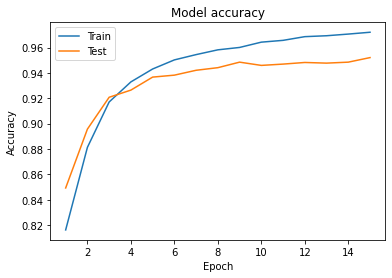
\includegraphics[width=.48\textwidth]{ModelSelection/selectedModelAcc.png} 
		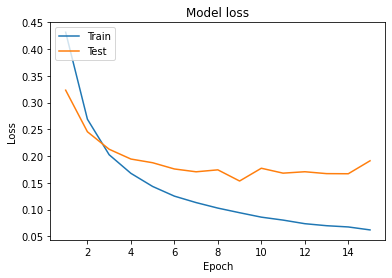
\includegraphics[width=.48\textwidth]{ModelSelection/selectedModelLoss.png} 
	\end{minipage}
	\caption{\textbf{Accuracy and loss function for the binary model:} The right figure shows the model's accuracy on training and validation data during 15 epochs, and the left figure shows the loss function values at different epochs.}
	\label{ModelSelection}
\end{figure}
\subsubsection*{Second case: 10-fold CV with unknown interactions}
In this case, we divide the set of all interactions (enhancive, degressive, and zeros of the first step) into 10 equal parts. We consider one part of the testing set and the other 9 parts as the training data set. Divide all the zeros in the previous step into 10 parts and add a 1 to 9 ratio to both testing and training sets. In the second case, the previous model's 10-fold CV procedure was trained with the least changes to predict the three classes. Besides, hyper-parameter, the number of epochs was determined. Figure
\ref{lastTripleModel} 

It shows the training process. The process of the accuracy of the model on training data increases steadily with the increase of epochs. Still, the model after epoch 9 reduces a constant and decreases the accuracy a little for testing data.

\begin{figure}[!h]
	%\centering
	\begin{minipage}{1\linewidth}
		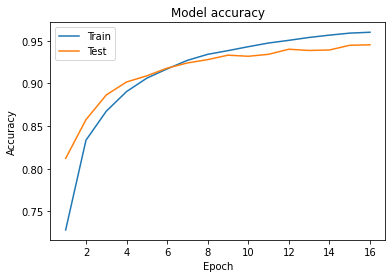
\includegraphics[width=.48\textwidth]{lastTripleModel/modelTripleACC.png}
		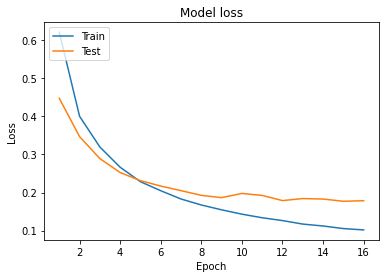
\includegraphics[width=.48\textwidth]{lastTripleModel/modelTripleLoss.png}
	\end{minipage}
	\caption{\textbf{Accuracy and loss function diagrams for the triple model:} The right figure shows the accuracy of the model on training and validation data during 16 epochs, and the left figure shows the loss function values at different epochs.}
	\label{lastTripleModel}
\end{figure}

\subsubsection*{Sub-sub heading for section}
Text for this sub-sub-heading\ldots
\paragraph*{Sub-sub-sub heading for section}


%
\[
E \bigl[Z_1(vT_x) \bigr]=
\int_0^{v\wedge
1}Z_0(uT_x)
\exp (\lambda_1)\,du .
\]
%
If we assume that sensitive cells follow a deterministic decay
$Z_0(t)=xe^{\lambda_0 t}$ and approximate their extinction time as
$T_x\approx-\frac{1}{\lambda_0}\log x$, then we can heuristically
estimate the expected value as
%
\begin{equation}\label{eqexpmuts}
\begin{aligned}[b]
&      E\bigl[Z_1(vT_x)\bigr]\\
&\quad      = \frac{\mu}{r}\log x
\int_0^{v\wedge1}x^{1-u}x^{({\lambda_1}/{r})(v-u)}\,du .
\end{aligned}
\end{equation}



\section*{Appendix}
Text for this section\ldots

%%%%%%%%%%%%%%%%%%%%%%%%%%%%%%%%%%%%%%%%%%%%%%
%%                                          %%
%% Backmatter begins here                   %%
%%                                          %%
%%%%%%%%%%%%%%%%%%%%%%%%%%%%%%%%%%%%%%%%%%%%%%

\begin{backmatter}

\section*{Acknowledgements}%% if any
Text for this section\ldots

\section*{Funding}%% if any
Text for this section\ldots

\section*{Abbreviations}%% if any
Text for this section\ldots

\section*{Availability of data and materials}%% if any
the code and data is available at GitHub page of \href{https://github.com/aminkhod/DDI-Project/tree/master/CNN\%20model\%20to\%20Recommend\%20Comperhancive\%20DDIs}{SNF-CNN code and data}


\section*{Ethics approval and consent to participate}%% if any
Text for this section\ldots

\section*{Competing interests}
The authors declare that they have no competing interests.

\section*{Consent for publication}%% if any
Text for this section\ldots

\section*{Authors' contributions}
Text for this section \ldots

\section*{Authors' information}%% if any
Text for this section\ldots

%%%%%%%%%%%%%%%%%%%%%%%%%%%%%%%%%%%%%%%%%%%%%%%%%%%%%%%%%%%%%
%%                  The Bibliography                       %%
%%                                                         %%
%%  Bmc_mathpys.bst  will be used to                       %%
%%  create a .BBL file for submission.                     %%
%%  After submission of the .TEX file,                     %%
%%  you will be prompted to submit your .BBL file.         %%
%%                                                         %%
%%                                                         %%
%%  Note that the displayed Bibliography will not          %%
%%  necessarily be rendered by Latex exactly as specified  %%
%%  in the online Instructions for Authors.                %%
%%                                                         %%
%%%%%%%%%%%%%%%%%%%%%%%%%%%%%%%%%%%%%%%%%%%%%%%%%%%%%%%%%%%%%

% if your bibliography is in bibtex format, use those commands:
\bibliography{bmc_article.bib}      % Bibliography file (usually '*.bib' )
\bibliographystyle{bmc-mathphys} % Style BST file (bmc-mathphys, vancouver, spbasic).

% for author-year bibliography (bmc-mathphys or spbasic)
% a) write to bib file (bmc-mathphys only)
% @settings{label, options="nameyear"}
% b) uncomment next line
%\nocite{label}

% or include bibliography directly:
% \begin{thebibliography}
% \bibitem{b1}
% \end{thebibliography}

%%%%%%%%%%%%%%%%%%%%%%%%%%%%%%%%%%%
%%                               %%
%% Figures                       %%
%%                               %%
%% NB: this is for captions and  %%
%% Titles. All graphics must be  %%
%% submitted separately and NOT  %%
%% included in the Tex document  %%
%%                               %%
%%%%%%%%%%%%%%%%%%%%%%%%%%%%%%%%%%%

%%
%% Do not use \listoffigures as most will included as separate files



\section*{Figures}
\begin{figure}[h!]
  \caption{Sample figure title}
\end{figure}

\begin{figure}[h!]
  \caption{Sample figure title}
\end{figure}

%%%%%%%%%%%%%%%%%%%%%%%%%%%%%%%%%%%
%%                               %%
%% Tables                        %%
%%                               %%
%%%%%%%%%%%%%%%%%%%%%%%%%%%%%%%%%%%

%% Use of \listoftables is discouraged.
%%
\section*{Tables}
\begin{table}[h!]
\caption{Sample table title. This is where the description of the table should go}
  \begin{tabular}{cccc}
    \hline
    & B1  &B2   & B3\\ \hline
    A1 & 0.1 & 0.2 & 0.3\\
    A2 & ... & ..  & .\\
    A3 & ..  & .   & .\\ \hline
  \end{tabular}
\end{table}

%%%%%%%%%%%%%%%%%%%%%%%%%%%%%%%%%%%
%%                               %%
%% Additional Files              %%
%%                               %%
%%%%%%%%%%%%%%%%%%%%%%%%%%%%%%%%%%%

\section*{Additional Files}
  \subsection*{Additional file 1 --- Sample additional file title}
    Additional file descriptions text (including details of how to
    view the file, if it is in a non-standard format or the file extension).  This might
    refer to a multi-page table or a figure.

  \subsection*{Additional file 2 --- Sample additional file title}
    Additional file descriptions text.

\end{backmatter}
\end{document}
